%%%%%%%%%%%%%%%%%%%%%%%%%%%%%%%%%%%%%%%%%%%%%%%%%%%%%%%%%%%%%%%%%%%%%%%%%%%%%%%%
% Template for USENIX papers.
%
% History:
%
% - TEMPLATE for Usenix papers, specifically to meet requirements of
%   USENIX '05. originally a template for producing IEEE-format
%   articles using LaTeX. written by Matthew Ward, CS Department,
%   Worcester Polytechnic Institute. adapted by David Beazley for his
%   excellent SWIG paper in Proceedings, Tcl 96. turned into a
%   smartass generic template by De Clarke, with thanks to both the
%   above pioneers. Use at your own risk. Complaints to /dev/null.
%   Make it two column with no page numbering, default is 10 point.
%
% - Munged by Fred Douglis <douglis@research.att.com> 10/97 to
%   separate the .sty file from the LaTeX source template, so that
%   people can more easily include the .sty file into an existing
%   document. Also changed to more closely follow the style guidelines
%   as represented by the Word sample file.
%
% - Note that since 2010, USENIX does not require endnotes. If you
%   want foot of page notes, don't include the endnotes package in the
%   usepackage command, below.
% - This version uses the latex2e styles, not the very ancient 2.09
%   stuff.
%
% - Updated July 2018: Text block size changed from 6.5" to 7"
%
% - Updated Dec 2018 for ATC'19:
%
%   * Revised text to pass HotCRP's auto-formatting check, with
%     hotcrp.settings.submission_form.body_font_size=10pt, and
%     hotcrp.settings.submission_form.line_height=12pt
%
%   * Switched from \endnote-s to \footnote-s to match Usenix's policy.
%
%   * \section* => \begin{abstract} ... \end{abstract}
%
%   * Make template self-contained in terms of bibtex entires, to allow
%     this file to be compiled. (And changing refs style to 'plain'.)
%
%   * Make template self-contained in terms of figures, to
%     allow this file to be compiled. 
%
%   * Added packages for hyperref, embedding fonts, and improving
%     appearance.
%   
%   * Removed outdated text.
%
%%%%%%%%%%%%%%%%%%%%%%%%%%%%%%%%%%%%%%%%%%%%%%%%%%%%%%%%%%%%%%%%%%%%%%%%%%%%%%%%

\documentclass[letterpaper,twocolumn,10pt]{article}
\usepackage{usenix2019_v3}

% to be able to draw some self-contained figs
\usepackage{tikz}
\usepackage{amsmath}

% inlined bib file
\usepackage{filecontents}

%-------------------------------------------------------------------------------
\begin{filecontents}{\jobname.bib}
%-------------------------------------------------------------------------------
@Book{arpachiDusseau18:osbook,
  author =       {Arpaci-Dusseau, Remzi H. and Arpaci-Dusseau Andrea C.},
  title =        {Operating Systems: Three Easy Pieces},
  publisher =    {Arpaci-Dusseau Books, LLC},
  year =         2015,
  edition =      {1.00},
  note =         {\url{http://pages.cs.wisc.edu/~remzi/OSTEP/}}
}
@InProceedings{waldspurger02,
  author =       {Waldspurger, Carl A.},
  title =        {Memory resource management in {VMware ESX} server},
  booktitle =    {USENIX Symposium on Operating System Design and
                  Implementation (OSDI)},
  year =         2002,
  pages =        {181--194},
  note =         {\url{https://www.usenix.org/legacy/event/osdi02/tech/waldspurger/waldspurger.pdf}}}
\end{filecontents}

%-------------------------------------------------------------------------------
\begin{document}
%-------------------------------------------------------------------------------

%don't want date printed
\date{}

% make title bold and 14 pt font (Latex default is non-bold, 16 pt)
\title{\Large \bf Indicus: Unchaining Byzantine Databases\\
 }

%for single author (just remove % characters)
\author{
{\rm Your N.\ Here}\\
Your Institution
\and
{\rm Second Name}\\
Second Institution
% copy the following lines to add more authors
% \and
% {\rm Name}\\
%Name Institution
} % end author

\maketitle

%-------------------------------------------------------------------------------
\begin{abstract}
%-------------------------------------------------------------------------------
Your abstract text goes here. Just a few facts. Whet our appetites.
Not more than 200 words, if possible, and preferably closer to 150.
\end{abstract}


%-------------------------------------------------------------------------------
\section{Introduction}
%-------------------------------------------------------------------------------



There is an increasing tension between the desire to share data online, and the security concerns it entails.
This paper asks the question: how can we enable \textit{mutually distrustful parties} to consistently and reliably
share data, while minimizing centralization?

The ability to share data online offers exciting opportunities.
\iffalse %% the medical record example is for privacy, more related to Obladi, but not BFT Tapir
In the medical domain, for
instance, cloud-based solutions for managing health record offer doctors increased fault-tolerance at lower
cost, and offer patient an easier path to share their medical
history with their entire treatment teams, even when on the road. Opportunities abound in other areas too.
\fi
In banking, systems like SWIFT enable financial institutions to quickly and accurately receive information
such as money transfer instructions; and in manufacturing, online data sharing can improve accountability
and auditing amongst the globally distributed supply chain.

Increased data sharing, however, raises questions of how to \textit{decentralize trust}.
\iffalse
Even when medical records are
encrypted or anonymized, cloud providers or dishonest applications may be able to acquire
sensitive information: for example, tracking the charts accessed by an oncologist can reveal not only whether
a patient has cancer, but also, depending on the frequency of accesses (e.g., the frequency of chemotherapy
appointments), indicate the cancers type and severity.
\fi
Banking institutions must currently place their trust
in the centralized SWIFT’s network to issue payment orders. Sometimes there is even no identifiable source of
trust. Consider the supply chain for the latest iPhone: it spans three continents, and hundreds of different
contractors~(https://www.apple.com/supplier-responsibility/pdf/Apple-Supplier-List.pdf); neither Apple nor these contractors trust each other, yet all must be willing to agree and share
information about the construction of the same product.


\iffalse %% Yunhao has removed the medical record example
\Yunhao{If I understand correctly, the medical record example is for privacy,
  the banking and the manufacturing example are for trust.
  I can see how BFT solves the later by decentralizing trust, but I cannot
  see how BFT solves the privacy problem. The access pattern of each transaction is visible to all parties.}
\fi

Recognizing this challenge by both the research and industry communities,
much effort has focused
on enabling shared computation between mutually distrustful parties, in the context of byzantine
fault tolerance (BFT), and blockchains.
Systems proposed in the literature of BFT[][] provide the abstraction of
a totally ordered log; the log is agreed upon by the $n$ participants in the system, of which at most $f$ can misbehave.
Each participant executes operations that may touch one to multiple objects in the log.
In the blockchain world,
Bitcoin and Ethureum have become popular distributed computing platforms
providing the same log abstraction and
aiming for decentralizing trust.
Furthermore, Microsoft Azure has launched projects[] that leverage these blockchain platforms and extend the digital transformation
beyond the companies' four walls in a supply chain.

%\Yunhao{This is the first time we mention transactions. I think we should distinguish 2 groups of research: BFT consensus and BFT transactions.}

This paper argues that there exists a fundamental mismatch between the implementation of %the abstraction of
a totally ordered log and the reality of much large-scale distributed processing. Many large-scale distributed
systems consist primarily of unordered and unrelated operations.
For example,
%Alice’s surgery need not be ordered with respect to Bob’s X-rays; likewise,
a product supply chain consists of many concurrent steps
that do not require ordering. Imposing an ordering on non-conflicting operations is not only often
unnecessary, but costly: participants in the shared computation must vote to order operations, store the full state of
the system, and replay the full log for auditing.

While there exists work on mitigating this scalability bottleneck
through sharding~\cite{}, the latent total order requirement introduces unnecessary coordination overhead, as
coordination is performed twice, at the level of individual shards, and across shards. Callinicos~\cite{} and
Omniledger~\cite{}, for instance, runs a full BFT protocol for every operation. This is especially problematic
when workloads are geo-replicated~\cite{}, or when, as in BFT, the replication factor is high.
%\Yunhao{I can see these two are examples of imposing ordering, but cannot see whether they are examples of twice coordination.}
Further, these systems
support transactions under the assumption that their read and write operations are known a priori, which
limits the set of applications that they can support.

As another research trend of mitigating the scalability bottleneck, 
EPaxos[], TAPIR[] and CURP[] only consider the ordering between potentially conflicting operations,
instead of commutative operations.
However, these systems assume the crash-failure model and are non-trivial to be extended to the Byzantine model,
so that they cannot directly solve the problem of data sharing among mutually distrustful parties.

Existing research, in essence, is either attempting to build concurrency control and sharding
functionalities over BFT replication, or integrating these functionalities into a crash-failure replication protocol.
%Existing research, in essence, is attempting to add database-like transactions and sharding
%functionality to a byzantine fault tolerant totally ordered log. We propose instead to flip the problem on its
%head by adding BFT to an efficiently shardable replicated database.
In this paper, we will show how to build these desiring functionality inside a BFT replication protocol.
Specifically, our goal is to \textit{provide the illusion of a centralized shared
log, rather than the non-scalable reality of a totally ordered log.}




%-------------------------------------------------------------------------------
\section{Indicus}
%-------------------------------------------------------------------------------
In the following we outline the Architecture and Protocols of Indicus, the first highly scalable database that tolerates both byzantine clients and replicas.
%-------------------------------------------------------------------------------
\subsection{Architecture}
%-------------------------------------------------------------------------------
Indicus follows a traditional optimistic concurrency control architecture as shown in Figure ~\ref{fig:Figure1}. Clients speculatively execute their Transactions, issuing remote reads when necessary and buffering writes locally. As Clients execute their own Transactions they need not declare their read/write keys or values preemtively, but rather may conduct interactive Transactions, the most general Transaction model. Since execution is speculative and Clients are unaware of potential concurrency, they must validate their Transactions for Isolation correctness in order to be able to Commit. Intuitively, if there are no conflicting concurrent Transactions and a Client observed a consistent snapshot of the distributed Database state then it may commit, and otherwise it must abort or retry. Lastly, Transactions may span multiple shards, and hence the Commit/Abort decisions of each shard must be aggregated in a Two Phase Commit manner in order to finalize a safety appropriate result. Most notably, in Indicus not just exeuction is Client driven but the entire Transaction life cycle, thus maximizing scalability and fairness while putting each Client in charge of its own liveness.
In the following we describe our Fault Model and define corresponding Transactional guarantees. We then outline the protocols for Execution, Validation and Writeback respectively.

\begin{figure*}
\begin{center}
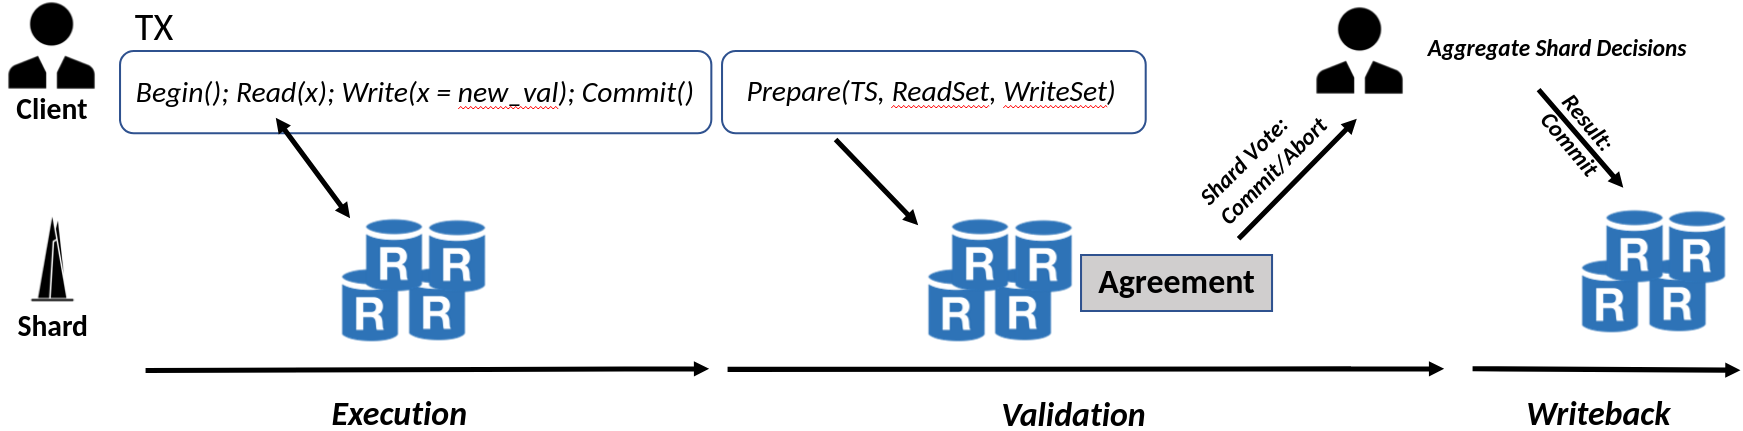
\includegraphics[width= \textwidth]{./figures/LC.png}
\end{center}
\caption{Transaction Lifecycle}
\label{fig:Figure1}
\end{figure*}

%-------------------------------------------------------------------------------
\subsection{Model and Definitions}
%-------------------------------------------------------------------------------

\subsubsection{System Model}
We assume a partitioned Database where data objects are spread uniformly across shards (randomly or based on locality). For fault tolerance we assume that each Shard contains 5f+1 replicas where f is the number of (static) faulty or compromised replicas. A faulty replica may behave in Byzantine fashion, i.e. in addition to crashing or omitting messages it may send arbitrary messages and deviate from prescribed protocols in any way.
We denote any participant (replica or client) that follows the protocol as \textit{honest}, while faulty participants are dubbed \textit{byzantine}. We assume there may exist a finite but unbounded number of byzantine Clients that may deviate from the protocol arbitrarily. 
 We further assume a strong, but static adversary that can coordinate the faulty participants 
 We do, however, assume the existance of sufficiently hard cryptographic primitives that allow for private/public key signatures and collision-resistant hashes that cannot be compromised by byzantine participants. We denote a signed message $m$, signed by principal $p$ as $\langle m \rangle_{\sigma p}$.
 
We make no assumption on network synchrony in order to maintain safety, but in some cases may provide liveness  only when the network is synchronous and messages are delayed by no more than a fixed but potentially unknown window. Unlike traditional State Machine Replication protocols in which the liveness of all Clients is correlated with the fate of the system (or often more specifically a leader), our system guarantees liveness not on a system basis, but on a per client basis. Concretely, we only guarantee liveness to clients that follow the protocol and conversely an honest client only loses liveness (even in an asynchronous setting) when it intertwines its fate with byzantine clients.

Application services may restrict the influence of Byzantine Clients on the Database state by authentication and enforcing access control. Beyond these measures, byzantine Clients that follow the protocol are indistinguishable from honest clients and may read and write at their leisure. While potential damage to the Database state cannot be avoided, it can be re-traced by auditing the Transaction logs.
 
\subsubsection{System properties}
We offer Clients an interactive Transaction interface that implements ACID transactions. While all ACID guarantees may be violated by individual byzantine Replicas, the system maintains the illusion of an ACID compliant state to all honest Clients.
Moreover, we guarantee to Clients that the Database is \textit{byzantine Serializable} as defined below. Intuitively this Isolation level guarantees that all honest Clients experience the Database as if there serializable. In order to formally capture this we lay some ground work: \footnote{Defs for commands etc in accordance with BFT DUr. cite}

Let $Op =  \{r, w\} \times K \times V $ and $Dec = \{Commit, \,Abort\}$ be the sets of possible operations and decisions respectively, where $K$ is the set of existing data items (keys) and $V$ the range of possible values. A \textit{request} $req \in (Op \cup Dec) \times C$ maps any such operation or decision to the issuing Client from set $C$. We denote with $Hon \subseteq C$ the subset of honest Clients. 

\textbf{History H.} Informally, a \textit{H} contains the operations (read/write) and decisions (commit/abort) of every transaction issued in the system. Formally, we define a \textit{history H} as a finite sequence of requests.

We define a projection $H|_c$ as the subsequence of requests in $H$ that were issued by Client $c$. A sequence of requests $s = req_i \dots req_{i+t}$ in $H|_c$ form a \textit{Transaction} if $req_i$ is the first request by Client $c$ or $req_{i-1} \in Dec \times c$, and if $req_{i+t} \in Dec \times c$.

We further define:

\textbf{Honest History H(P).} Given protocol P, A \textit{history H} is \textit{honest} if it was generated by participants who all follow P. I.e. concretely, $H(P) \equiv H = H|_{Hon}$.
and

\textbf{Honest-View Equivalent.} A \textit{history H} is honest-view equivalent to a $history H'$ if the Operations and Decisions of all honest Clients are the same and if the final writes are the same.

\textbf{Byz-I} Given a protocol $P$ and an isolation level $I$:
A history H is \textit{byzantine-I} if there exists an honest history \textit{H'} such that H is honest-view equivalent to H' and H' satisfies I. 

Thus, informally a byzantine Isolation level states that the state that honest Clients experience must be explicable by an execution in which all participants were honest.
This definition captures the requirements for any byzantine tolerant protocol that strives to maintain Isolation level I.

We further define some progress properties to limit the influence Byzantine Clients have on system throughput. These will be motiviating factors that we will return to in order to justify our choice of 5f+1 replicas as well as the use of an Optimistic Concurrency Control over a Locking based schema. We later outline an alternative design using 3f+1 replicas that does not maintain this property. 




%-------------------------------------------------------------------------------
\subsection{Execution}
%-------------------------------------------------------------------------------
%-------------------------------------------------------------------------------
\subsection{Validation}
%-------------------------------------------------------------------------------

%-------------------------------------------------------------------------------
\subsection{Concurrency Control}
%-------------------------------------------------------------------------------
 - Optimization: retries
 - Dependency resolution
%-------------------------------------------------------------------------------
\subsection{Consistent logging.}
%-------------------------------------------------------------------------------



%-------------------------------------------------------------------------------
\subsection{Writeback and Multi-shard 2pc}
%-------------------------------------------------------------------------------

- Optimization: Single shard logging
%-------------------------------------------------------------------------------
\subsection{Failures}
%-------------------------------------------------------------------------------
- Fallback: election, resolution, subtelties with mvtso, necessity even without dependencies.

%-------------------------------------------------------------------------------
\subsection{Low Cost mode}
%-------------------------------------------------------------------------------
3f+1 if not defending against byz colluders
OCC if not worried about reads aborting


%-------------------------------------------------------------------------------
\section{Implementation and Evaluation}
%-------------------------------------------------------------------------------


%-------------------------------------------------------------------------------
\section{Limitations}
%-------------------------------------------------------------------------------
As is inherent to any Optimistic Execution and Concurrency Control, Indicus is vulnerable to highly congested workloads. When contention on select objects is high, concurrent execution of Transactions must yield in the abort of some Transactions during Validation in order to maintain the Database Isolation guarantees. Note however, that when clients are in charge of execution, a pessimistic concurrency control solution such as two-phase-locking would incur an equal amount of deadlocks which would require resolution. The observation to make is that any system that conducts execution at the client application side speculates on concurrency. This however we stipulate, is unavoidable when trying to scale a system to the number of users rather than replica processing power. The traditonal ways to avoid the abort rate conundrum is to either restrict the transaction model, which in turn weakens the general applicability of the protocol, or to delegate execution to replicas and utilize State Machine Replication to serialize Transactions. Indicus does not make these concessions in order to offer interactive Transactions and remain scalable. A workload that exhibits low commutativity and high contention should therefore refrain from adopting our system.

Similarly, as is the case in any transaction protocol, Indicus is vulnerable to ddos attacks by byzantine participants. A byzantine clients only opportunity at subverting progress for honest users is to artificially increase congestion. When such a client has unrestricted access control it may do so strategically iff it has control over the network. If it does not, it cannot reliably gain knowledge about concurrent transactions before they pass the validation step and must resort to flooding based attacks. Defense against such attacks is out of scope in our work, but is disincentivised as participants can be held accountable for their actions in a closed membership setting.


%-------------------------------------------------------------------------------
\section{Related Work/Comparison}
%-------------------------------------------------------------------------------
A lot of recent effort has gone into designing high throughput and low latency databases that leverage synergies between transaction and replication layer to squeeze out any last performance. The recently proposed TAPIR transaction protocol leverages redundancy between transaction ordering and replication ordering to reduce total roundtrips, thus reducing latency in wide area networks. TAPIR shares several similarities with our system, most notably the absence of a leader and the resulting unordered validation structure. TAPIR too, leverages optimistic concurrency control to allow for concurrency among commutative transactions. When congestion is high however, throughput and tail latency worsen as abort rate grows. Janus avoids transaction aborts by dynamically re-ordering conflicting transactions. This however, is made possible by assuming one-shot transactions, i.e. fixed read/write keys, and thus reduces the application generality. Another DB, Carousel similarly assumes a restricted Transaction model in order to parallelize execution and validation. While all of these databases offer low latency replication, they are fundamentally limited to tolerating crash-failures. This strong failure assumption makes them less secure and not suitable for storing mission-critical, financial or highly sensitive data. 
With the surge in Blockchain interest Byzantine Fault Tolerant (BFT) protocols are experiencing a second Spring. While originally developed to tolerate arbitrary bugs, these protocols find increasing importance in settings where participants are untrusted or malicious. Permissioned Blockchains, organized by a consortium of registered participants can use traditional BFT State Machine Replication (SMR) protocols in order to achieve agreement. Starting with PBFT, there have been numerous adaptations such as FaB or Generalized byzantine Paxos, and most notably Zyzzyva which leverages speculative execution and a semi-client driven protocol to reduce latency. SBFT modifies PBFT to scale to large replication degrees by utilizing collectors, threshold signatures and a fast path akin to Zyzzyva. Aardvark states the importance of robustness against byzantine failures and takes measures to increase the rate of leader rotation.
Nevertheless, all protocols derived from the PBFT family suffer from the leader bottleneck as well as enforcing a total order even on commutative operations. Biblos achieves leaderless SMR by leveraging a non-skipping timestamp protocol. It furthermore allows for commutative Transactions to be executed in parallel at the cost of requiring read/write key sets to be known in advance. In order to preserve liveness however Bilbos falls back to a PBFT resolution. Q/U too, offers leaderless agreement via Qurorums for a limited read/write interface, but fails to terminate under contention. H/Q improves upon Q/U by adding PBFT fallback path under contention. Liskov et Al further explore byzantine Quorum protocols for a Read/Write interface, giving special attention to bounding the effects of byzantine clients. 
While the literature on BFT state machine replication is extensive, the efforts to offer a transactional interface for BFT is scarce. SMR itself can be utilized as a straw-man system to implement pre-defined Transactions (one-shot or stored procedures) by enforcing a common total order  in which replicas will execute the transactions. 
HRDB offers a dedicated BFT Database, but assumes a trusted shepheard layer, thus not being truly BF resilient
Byantium offers Snapshot Isolation for Transactions by re-purposing PBFT as atomic broadcast. It executes requests only at a primary and uses replicas to validate results in the total order defined by the SMR protocol. Augustus implements mini-transactions, a limited TX model that declares all operations before execution. It offers scalability via partitioning and achieves consistency within partitions by utilizing atomic broadcast. Whiile Augustus assumes an optimistic execution model that allows for aborts under concurrency, its follow up work Callinicos implements a locking scheme in order to avoid Transaction aborts. To do so efficiently it resorts to a limited transaction model that requires knowledge of read/write sets and otherwise locks an entire partition in order to guarantee mutual exclusion, thus voiding any concurrency. BFT Deferred update replication adopts an interactive OCC transaction model comparable to ours, allowing execution to be speculative at clients. However, it uses PBFT atomic broadcast to enforce SMR on validation, thus resorting to a leader, and totally ordering all requests. It moreover does not extend to multiple shards.
Chainspace and Omniledger implement blockchain sharding by layering 2PC and atomic broadcast (within shards) for UTXO transactions. Rapidchain offers efficient sharding for a permissionless system. 

\cite{kotla2007zyzzyva}

%-------------------------------------------------------------------------------
\section{Conclusion}
%-------------------------------------------------------------------------------


%-------------------------------------------------------------------------------
\section*{Acknowledgments}
%-------------------------------------------------------------------------------

The USENIX latex style is old and very tired, which is why
there's no \textbackslash{}acks command for you to use when
acknowledging. Sorry.

%-------------------------------------------------------------------------------
\section*{Availability}
%-------------------------------------------------------------------------------

USENIX program committees give extra points to submissions that are
backed by artifacts that are publicly available. If you made your code
or data available, it's worth mentioning this fact in a dedicated
section.

%-------------------------------------------------------------------------------
\bibliographystyle{plain}
\bibliography{ref}


%%%%%%%%%%%%%%%%%%%%%%%%%%%%%%%%%%%%%%%%%%%%%%%%%%%%%%%%%%%%%%%%%%%%%%%%%%%%%%%%
\end{document}
%%%%%%%%%%%%%%%%%%%%%%%%%%%%%%%%%%%%%%%%%%%%%%%%%%%%%%%%%%%%%%%%%%%%%%%%%%%%%%%%

%%  LocalWords:  endnotes includegraphics fread ptr nobj noindent
%%  LocalWords:  pdflatex acks